% presentation/slides/10_resultats.tex
\begin{frame}{Observations Numériques et Analyse d'Erreur}
    \begin{columns}[c]
        \begin{column}{0.5\textwidth}
            \centering
            % Remplacer par 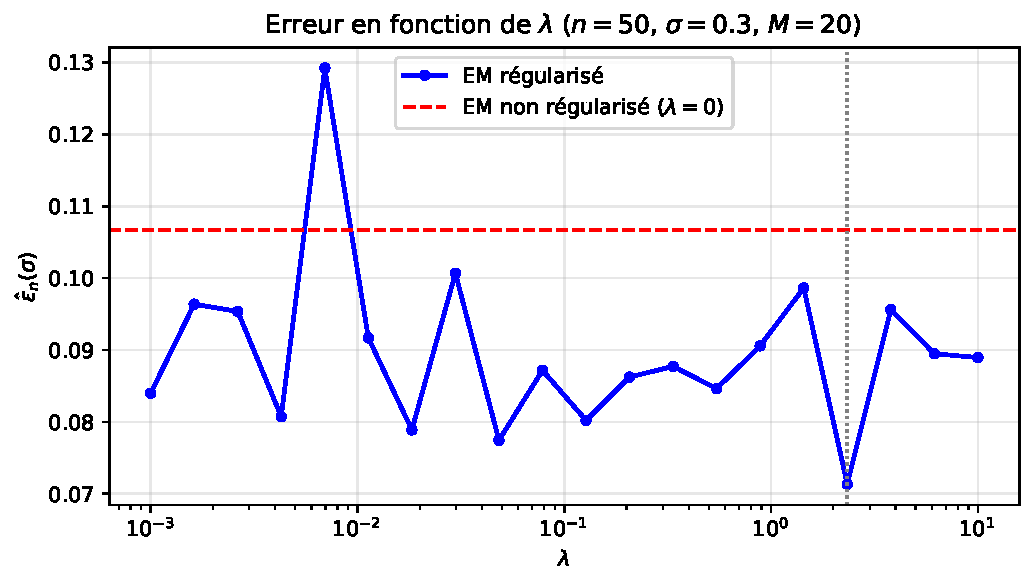
\includegraphics[width=0.85\textwidth]{figures/erreur_vs_lambda.pdf}
            \framebox{\begin{minipage}{0.85\textwidth}\centering\vspace{1.0cm}\textcolor{DarkBeige}{\textbf{[ erreur_vs_lambda.pdf ]}}\\\small Compromis biais-variance sur $\lambda$\vspace{1.0cm}\end{minipage}}
        \end{column}
        \begin{column}{0.5\textwidth}
            \centering
            % Remplacer par 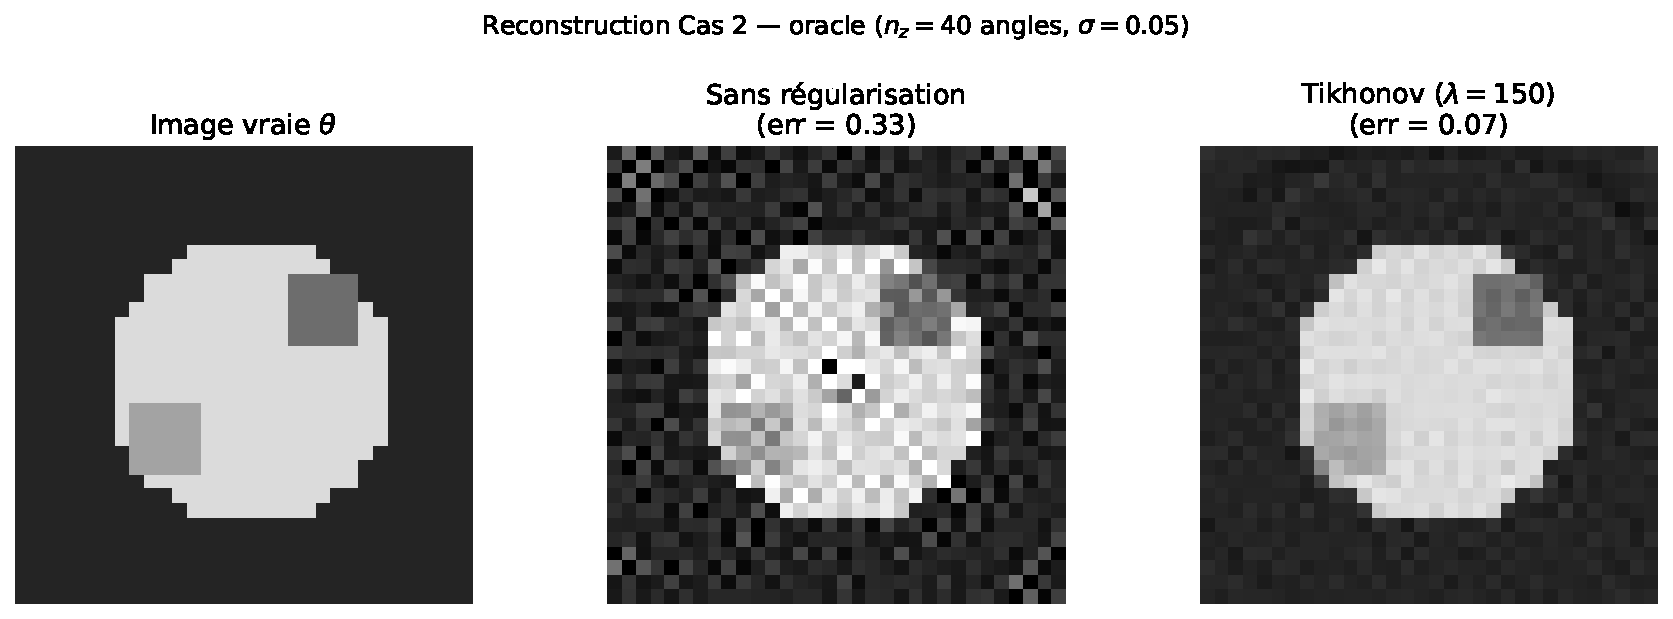
\includegraphics[width=0.85\textwidth]{figures/reconstruction_2d.pdf}
            \framebox{\begin{minipage}{0.85\textwidth}\centering\vspace{1.0cm}\textcolor{DarkBeige}{\textbf{[ reconstruction_2d.pdf ]}}\\\small Impact de la TV en 2D\vspace{1.0cm}\end{minipage}}
        \end{column}
    \end{columns}
    \vspace{0.3cm}
    \begin{center}
        \small \textbf{L'indispensable compromis :} Si $\lambda$ est trop faible, le bruit submerge l'image. Si $\lambda$ est trop fort, les détails structuraux fins s'estompent (biais élevé).
    \end{center}
\end{frame}